\documentclass{article}
\usepackage[utf8]{inputenc}
\usepackage{graphicx}
\usepackage{enumerate}
\usepackage{amsmath}
\usepackage{parskip}
\usepackage{siunitx}

\usepackage{geometry}
 \geometry{
 a4paper,
 total={170mm,257mm},
 left=20mm,
 top=20mm
 }

\title{TP: Cellular Network Planning on a 2D Map}
\author{Markus Säynevirta}
\date{June 2022}

\begin{document}

\thispagestyle{plain}

\large
\textbf{RIO207 - Ingénierie radio}

\large
TP: Cellular Network Planning on a 2D Map\\
\textit{Markus Säynevirta}
\vspace{0.5cm}

\section{Pre-dimensioning based on pilot coverage}
\subsection{Link budget (question 1)}

In- and outdoor sensitivities were computed for the pilot signal as part of a link budget spreadsheet included in the exercise zip archive. Table \ref{tab:link_budget} presents an excerpt containing the sensitivity values for both coverage scenarios as well as cell radii computed for these same scenarios.

\begin{table}[!htb]
    \centering
    \begin{tabular}{|l|l|l|}
    \hline
    \multicolumn{3}{|c|}{\textbf{Sensitivities}} \\ \hline
    Sensitivity, indoor {[}dBm{]}          & -92.92  &                                       \\ \hline
    Sensitivity, outdoor {[}dBm{]}         & -107.92 &                                       \\ \hline
    \multicolumn{3}{|c|}{\textbf{Cell range}} \\ \hline
    MAPL indoor {[}dB{]}                   & 140.43  & given value                           \\ \hline
    MAPL outdoor {[}dB{]}                  & 155.43  & given value                           \\ \hline
    Hata A                                 & 134.35  & given value                           \\ \hline
    Hata B                                 & 38.98   &                                       \\ \hline
    Hata C                                 & 0.44    &                                       \\ \hline
    Cell range, indoor {[}km{]}            & 1.47    &                                       \\ \hline
    Cell range, outdoor {[}km{]}           & 3.56    &                                       \\ \hline
    \end{tabular}
\caption{An excerpt from the link budget.}
\label{tab:link_budget}
\end{table}

\subsection{Site coverage and number (question 2)}

Table \ref{tab:cell_numbers} presents the approximate numbers of cells in the two previously outlined deployment scenarios. These numbers have been computed by dividing the service area of \(\SI{100}{\kilo\metre\squared}\) with the area of the hexagonal cell calculated from the equation \(A_c = \frac{3 \sqrt{3} R^2}{8} \) and taking a ceiling function of the result.

\begin{table}[!htb]
    \centering
    \begin{tabular}{|l|l|}
    \hline
    \multicolumn{2}{|c|}{\textbf{Number of cells, indoor}} \\ \hline
    Cell area {[}km²{]}                    & 1.40                                        \\ \hline
    Number of cells                        & 72.00                                       \\ \hline
    \multicolumn{2}{|c|}{\textbf{Number of cells, outdoor}} \\ \hline
    Cell area {[}km²{]}                    & 8.25                                        \\ \hline
    Number of cells                        & 13.00                                       \\ \hline
    \end{tabular}
    \caption{Number of cells in the different deployment scenarios.}
    \label{tab:cell_numbers}
\end{table}

\section{Cell planning based on coverage}
\subsection{Site planning proposal (question 3)}
Figure \ref{fig:q3_pilot_coverage} present the proposed BS site layout and the resulting pilot coverage. The number of 10 deployed sites is somewhat lower than the lower bound of 13 gained in the link budget based coverage study.

\begin{figure}[!htb]
    \centering
    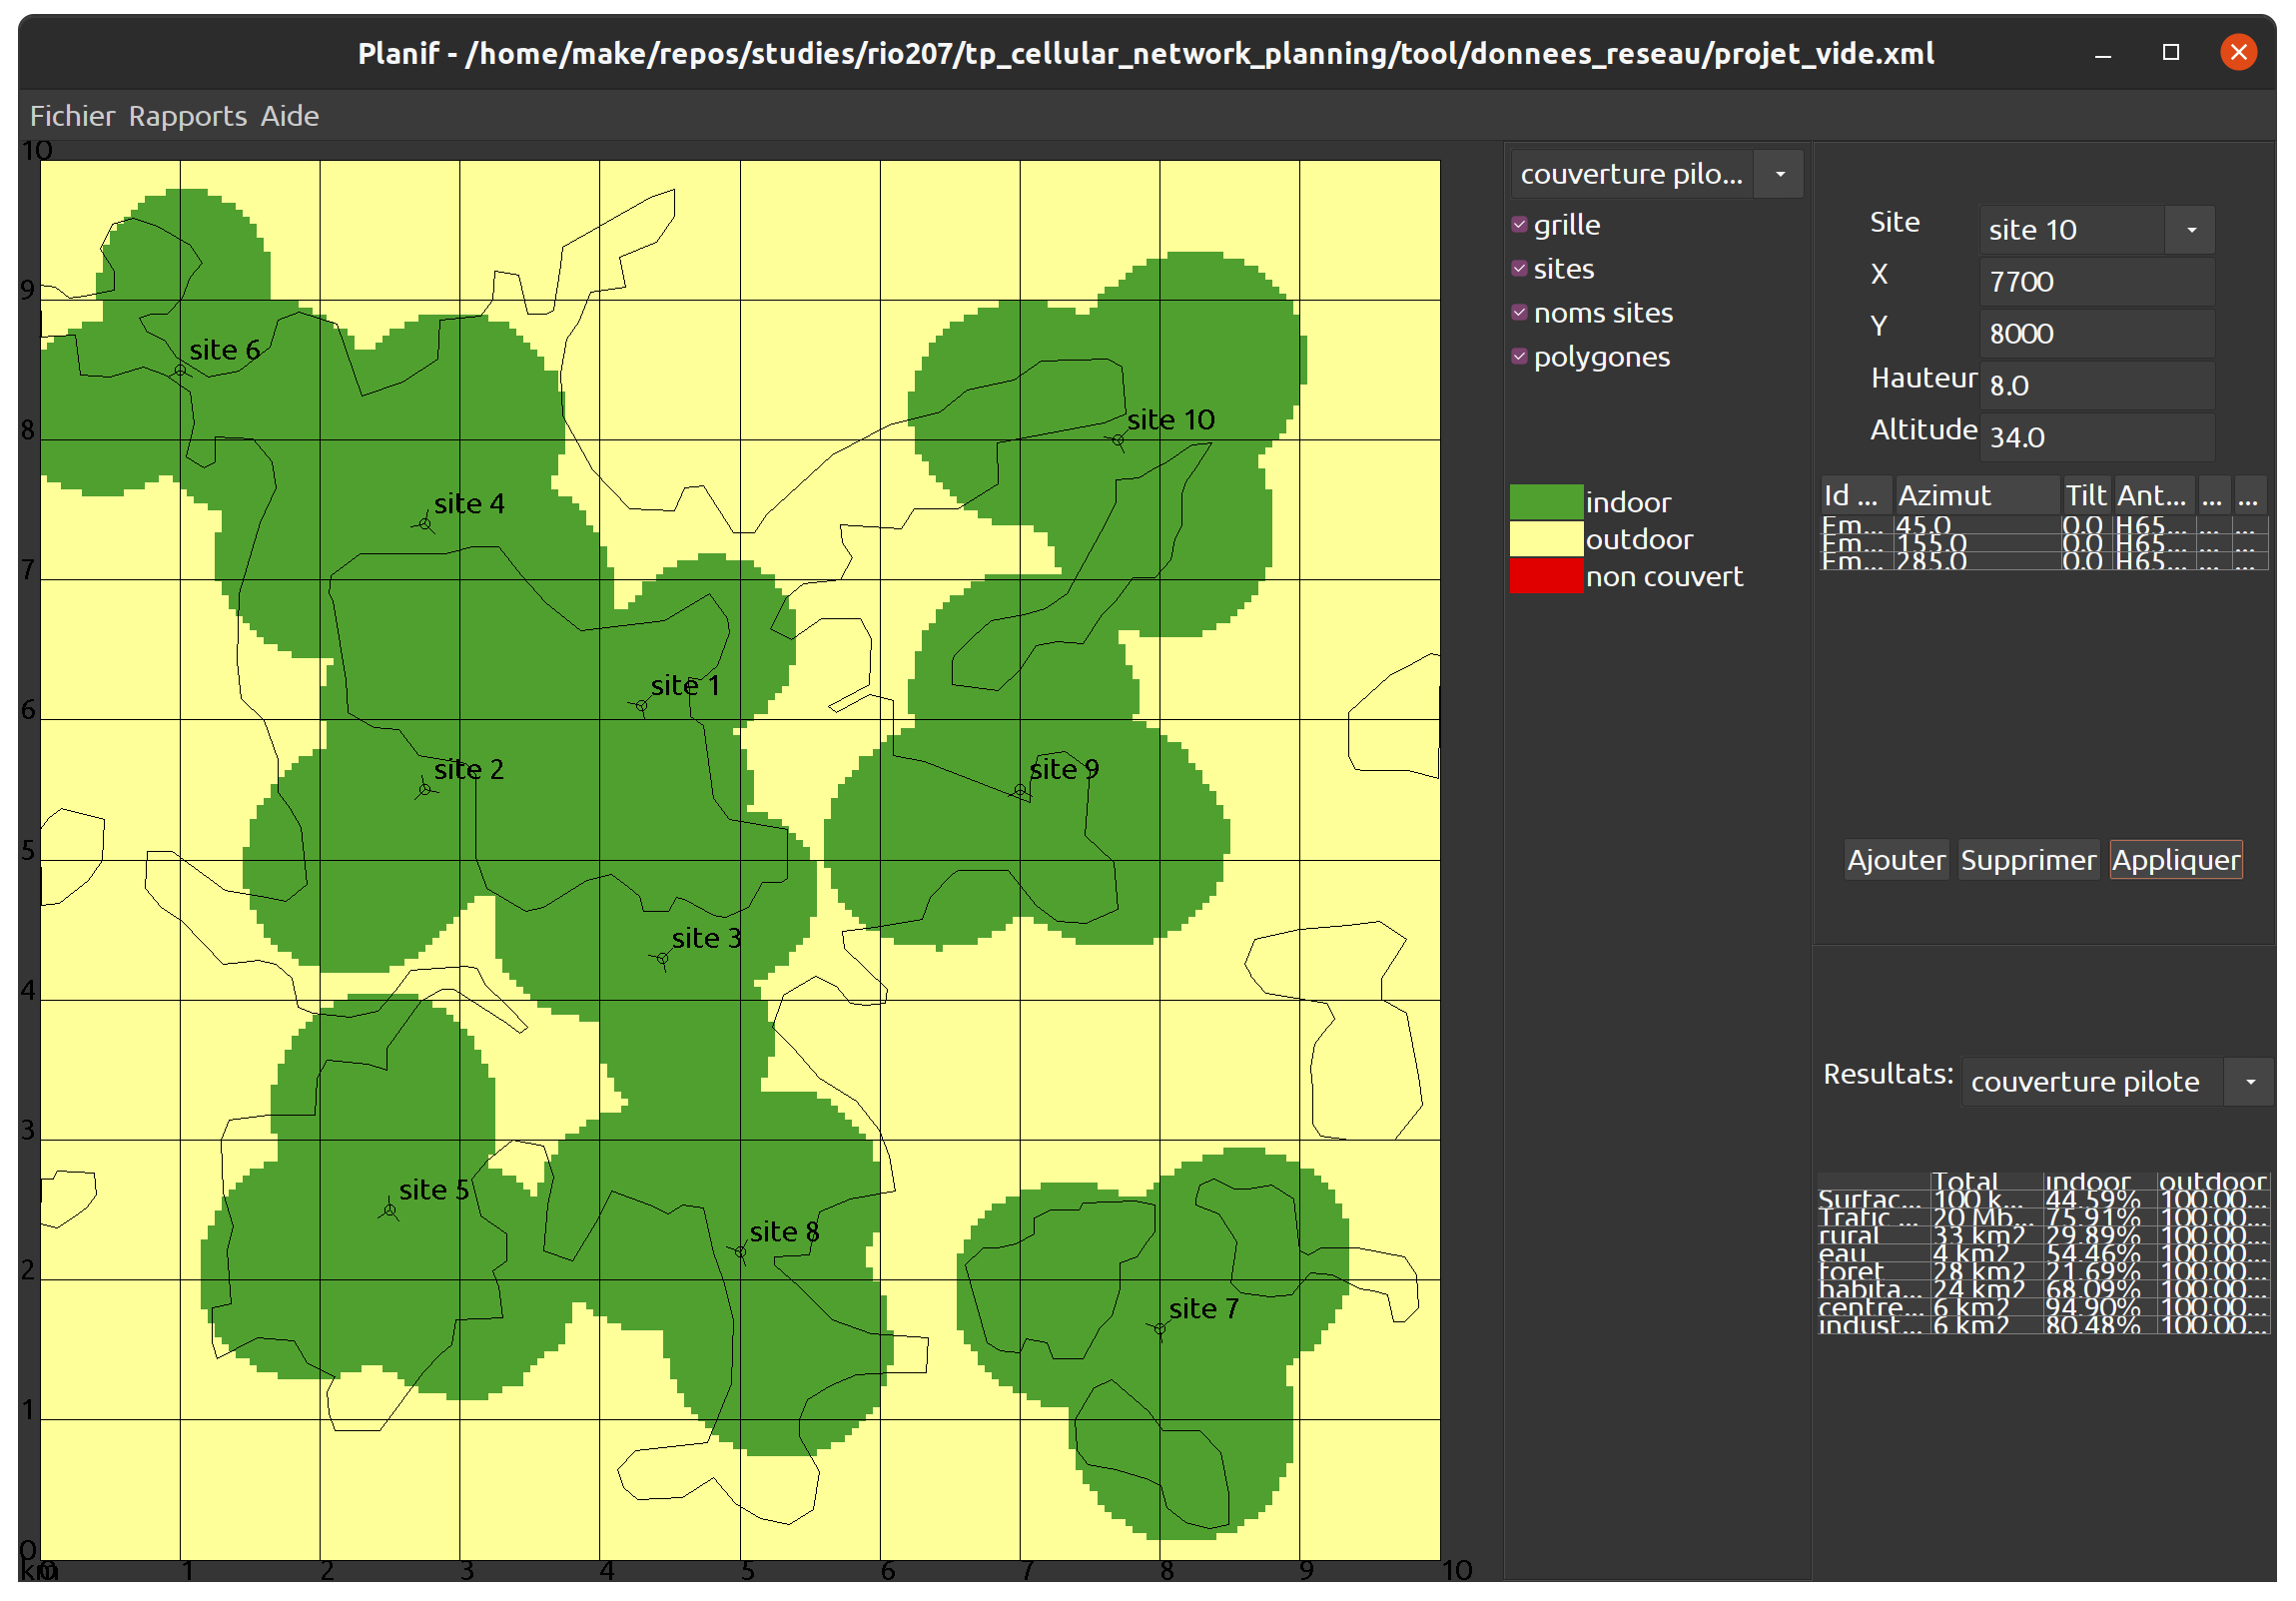
\includegraphics[width=12cm]{images/q3_pilot_coverage.png}
    \caption{Pilot coverage in the first deployment scenario.}
    \label{fig:q3_pilot_coverage}
\end{figure}

The cell positioning of the sites gives an outdoor geographic coverage of 100\ \% while the indoor coverage remains at 45\ \%.

\newpage
\subsection{Cell loading (question 4)}
Figure \ref{fig:q4_cell_loading} presents the resulting cell loading from the previously proposed BS site layout.

\begin{figure}[!htb]
    \centering
    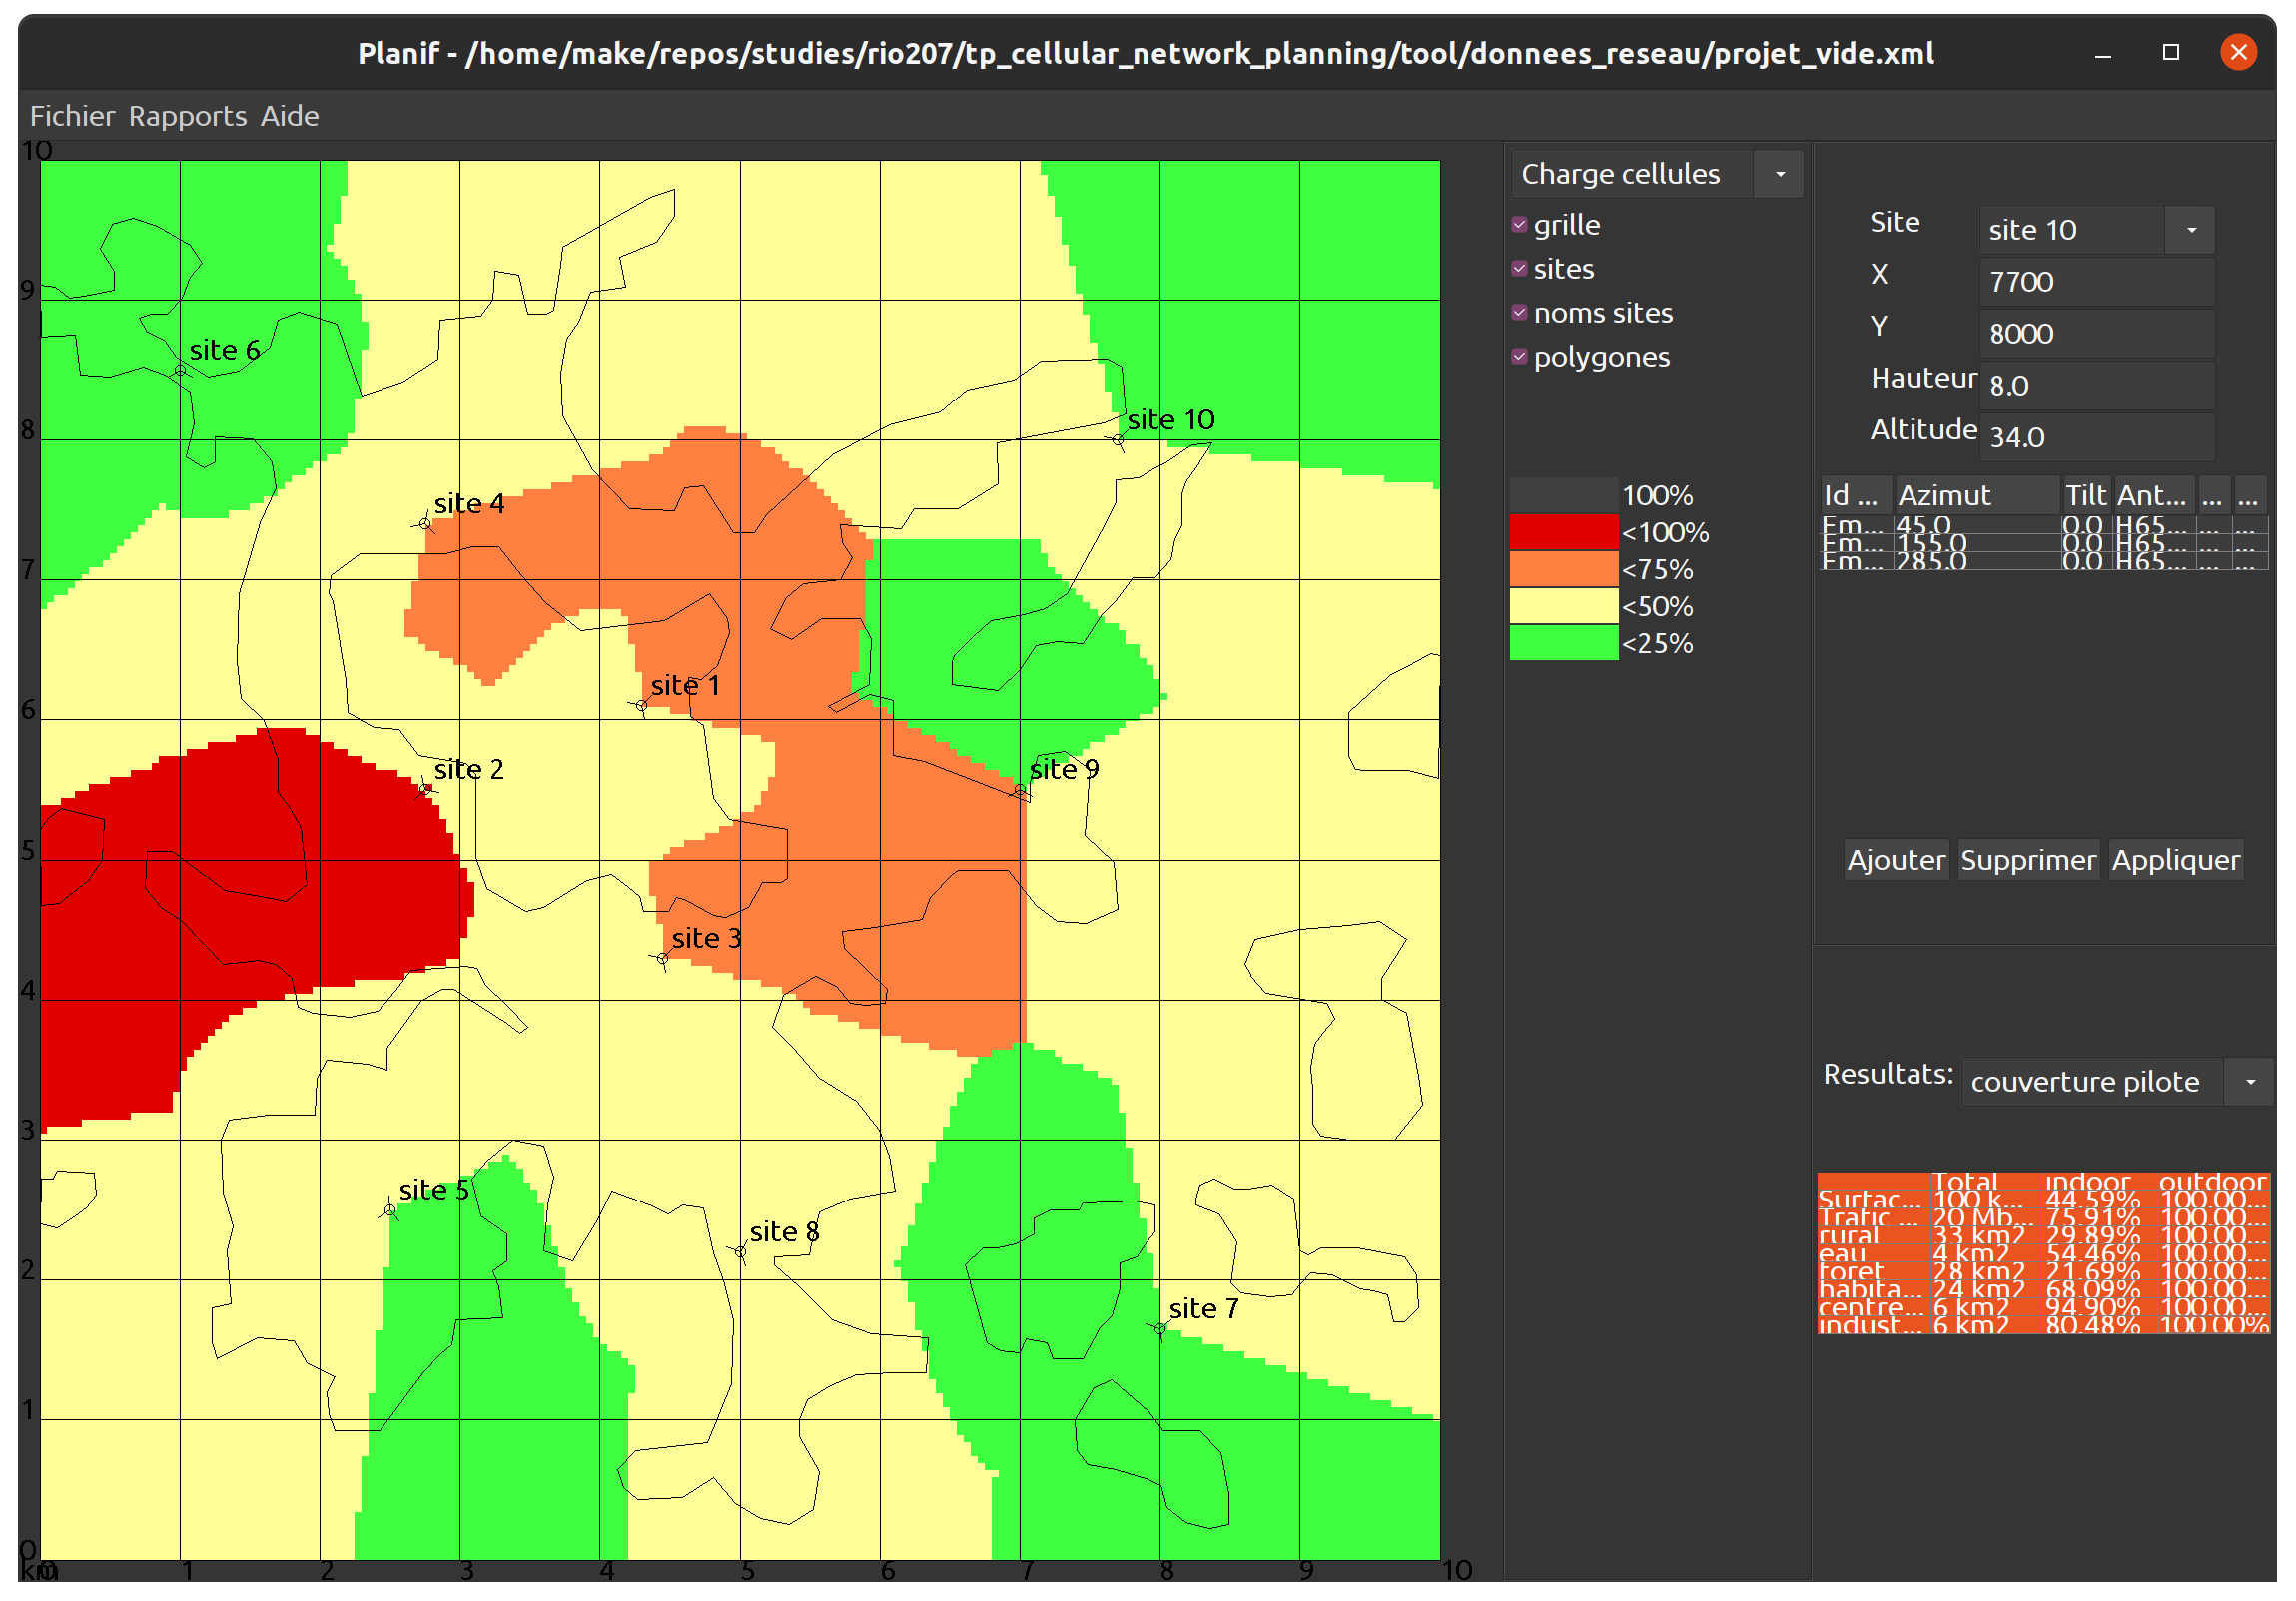
\includegraphics[width=12cm]{images/q4_cell_loading.png}
    \caption{Cell loading in the first deployment scenario.}
    \label{fig:q4_cell_loading}
\end{figure}

As can be seen from the figure, the cells in the most densely populated urban regions are the most loaded with figures ranging from \(< 75 \% - < 100 \%\). Higher site density helps though, and these regions remain still served overall, at least in terms of outdoor coverage. Based on the results of the simulation, 100\ \% of the outdoor traffic demand is being served.

\section{Capacity study}
\subsection{Pre-dimensioning based on cell capacity (questions 5 - 7)}
Evaluating approximate cell capacity requires us to solve SINR figures for each of the \(\SI{200}{\metre}\) radii concentric rings that the BS coverage area is divided into. SINR can be calculated from the equation

\begin{gather*}
    \mathrm{SINR} = P_{rx} - N - M_{\mathrm{interference}}
\end{gather*}

\(P_{rx}\) and \(N\) are the received signal power and noise power in the allocated bandwidth in \si{\deci\bel m}. \(M_{\mathrm{interference}}\) is the interference margin in \si{\deci\bel}. The figure for \(N\) can be taken from the previously computed link budget while \(\mathrm{M_{interference}}\) has been given in the exercise description. Received signal power can be computed from the equation

\begin{gather*}
    P_{rx} = \mathrm{EIRP_{dBm}} + G_{rx} - \mathrm{PL}
\end{gather*}

\(\mathrm{EIRP_{dBm}}\) and \(\mathrm{PL}\) are the transmitter's effectively isotropically radiated power and the path loss predicted by the Okumura-Hata propagation model, both in \si{\deci\bel m}. \(G_{rx}\) is the receiver antenna gain in \si{\deci\bel i}, which is in this case just 0.

The exact SINR figures have been computed in the spreadsheet included in the exercise zip archive.

Average data rate was computed from the throughputs solved for the different parts of the coverage area by taking an area-weighted harmonic mean

\begin{gather*}
    C_{mean} = \left( \frac{\sum\limits_{i=1}^n A_i C_i^{-1}}{\sum\limits_{i=1}^n A_i} \right)^{-1}.
\end{gather*}

The results are presented in table \ref{tab:data_rates}. The overall cell data rate is the mean multiplied by three and the number of required sites can be solved from the figure by dividing the service area with it and taking a ceiling function of the result. As we can see, the expected number of sites matches closely the lower bound for the number obtained from the link budget.

\begin{table}[!htb]
    \centering
    \begin{tabular}{l|l|}
    \hline
    \multicolumn{2}{|c|}{\textbf{Results}} \\ \hline
    \multicolumn{1}{|l|}{Average data rate {[}Mbps{]}} & 0.49 \\ \hline
    \multicolumn{1}{|l|}{Cell data rate {[}Mbps{]}}    & 1.48 \\ \hline
    \multicolumn{1}{|l|}{Number of sites}              & 14   \\ \hline
    \end{tabular}
    \label{tab:data_rates}
    \caption{Average data rate solved by taking a weighted harmonic mean. Number of BS sites has been calculated from the total cell data rate.}
\end{table}

\newpage
\subsection{Cell planning based on capacity (question 8)}

Figures \ref{fig:q8_pilot_coverage} and \ref{fig:q8_cell_loading} present the pilot signal coverage and cell loading of the second deployment scenario with a total of 16 BS sites.

Based on the results of the simulation, the chosen positioning gives an outdoor pilot coverage of 100\ \%. The network serves 100\ \% of the outdoor and 94\ \% of the indoor traffic demand.

\begin{figure}[!htb]
    \centering
    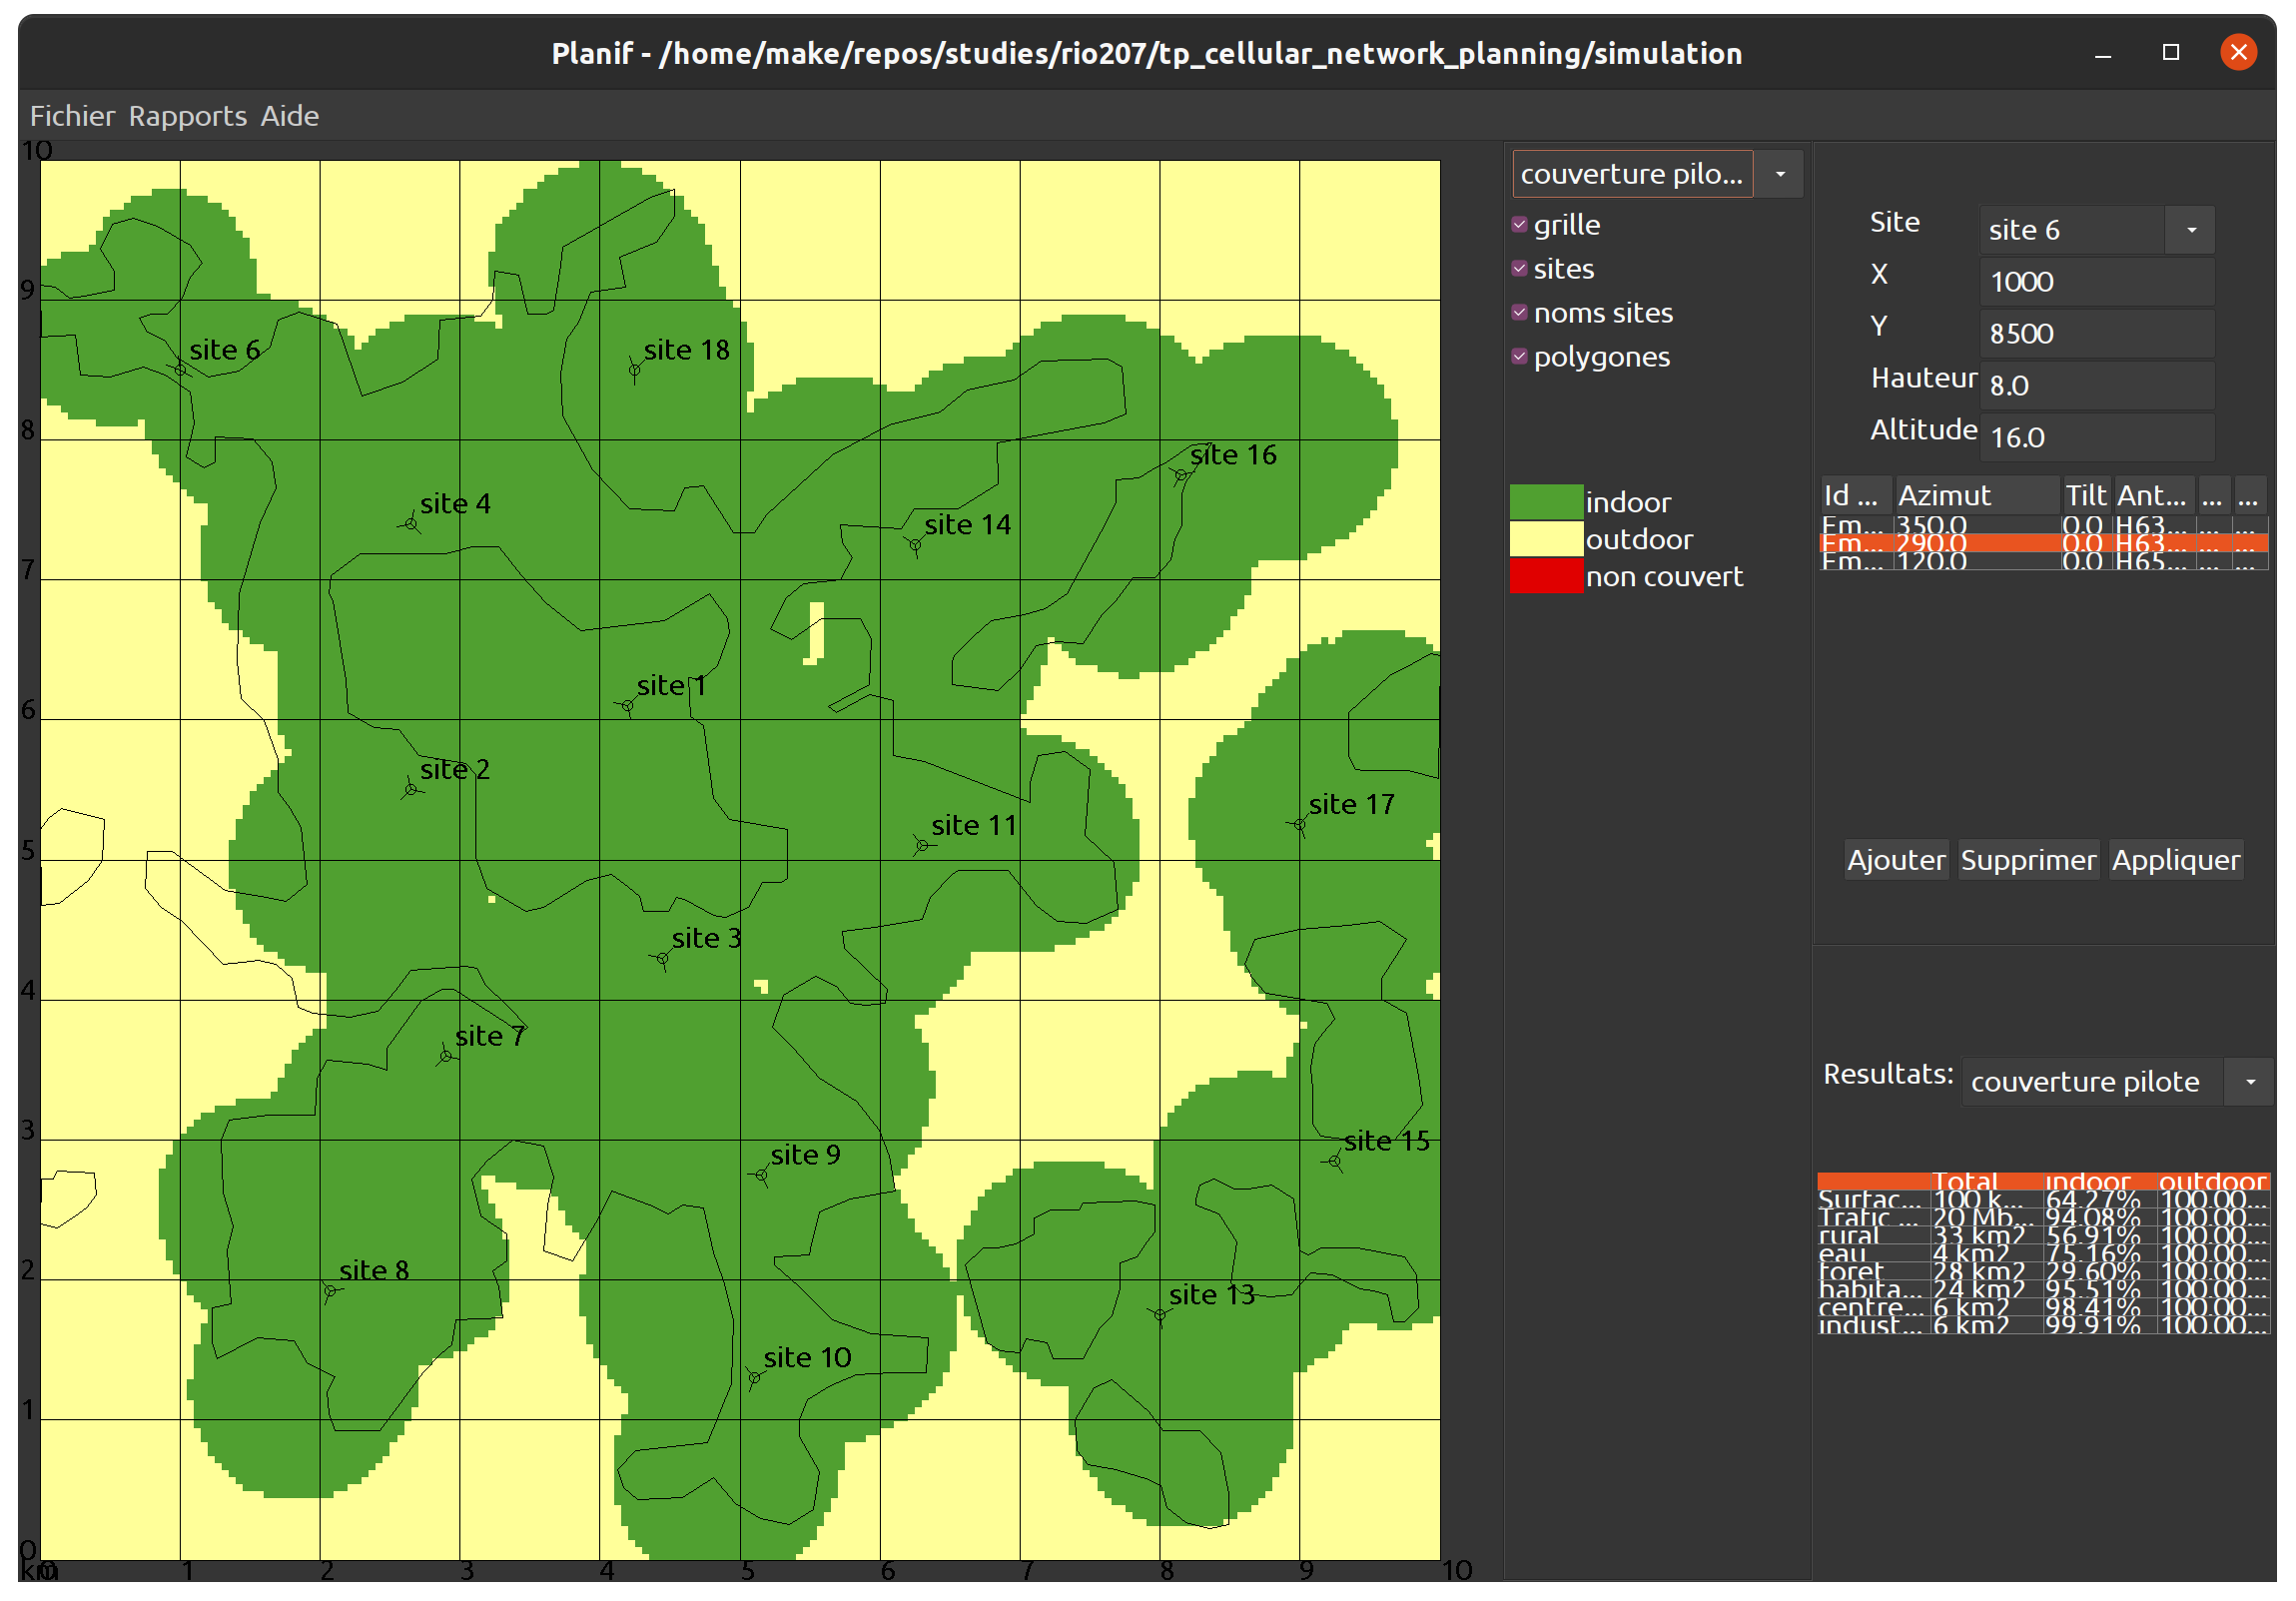
\includegraphics[width=12cm]{images/q8_pilot_coverage.png}
    \caption{Pilot coverage in the second deployment scenario.}
    \label{fig:q8_pilot_coverage}
\end{figure}

\begin{figure}[!htb]
    \centering
    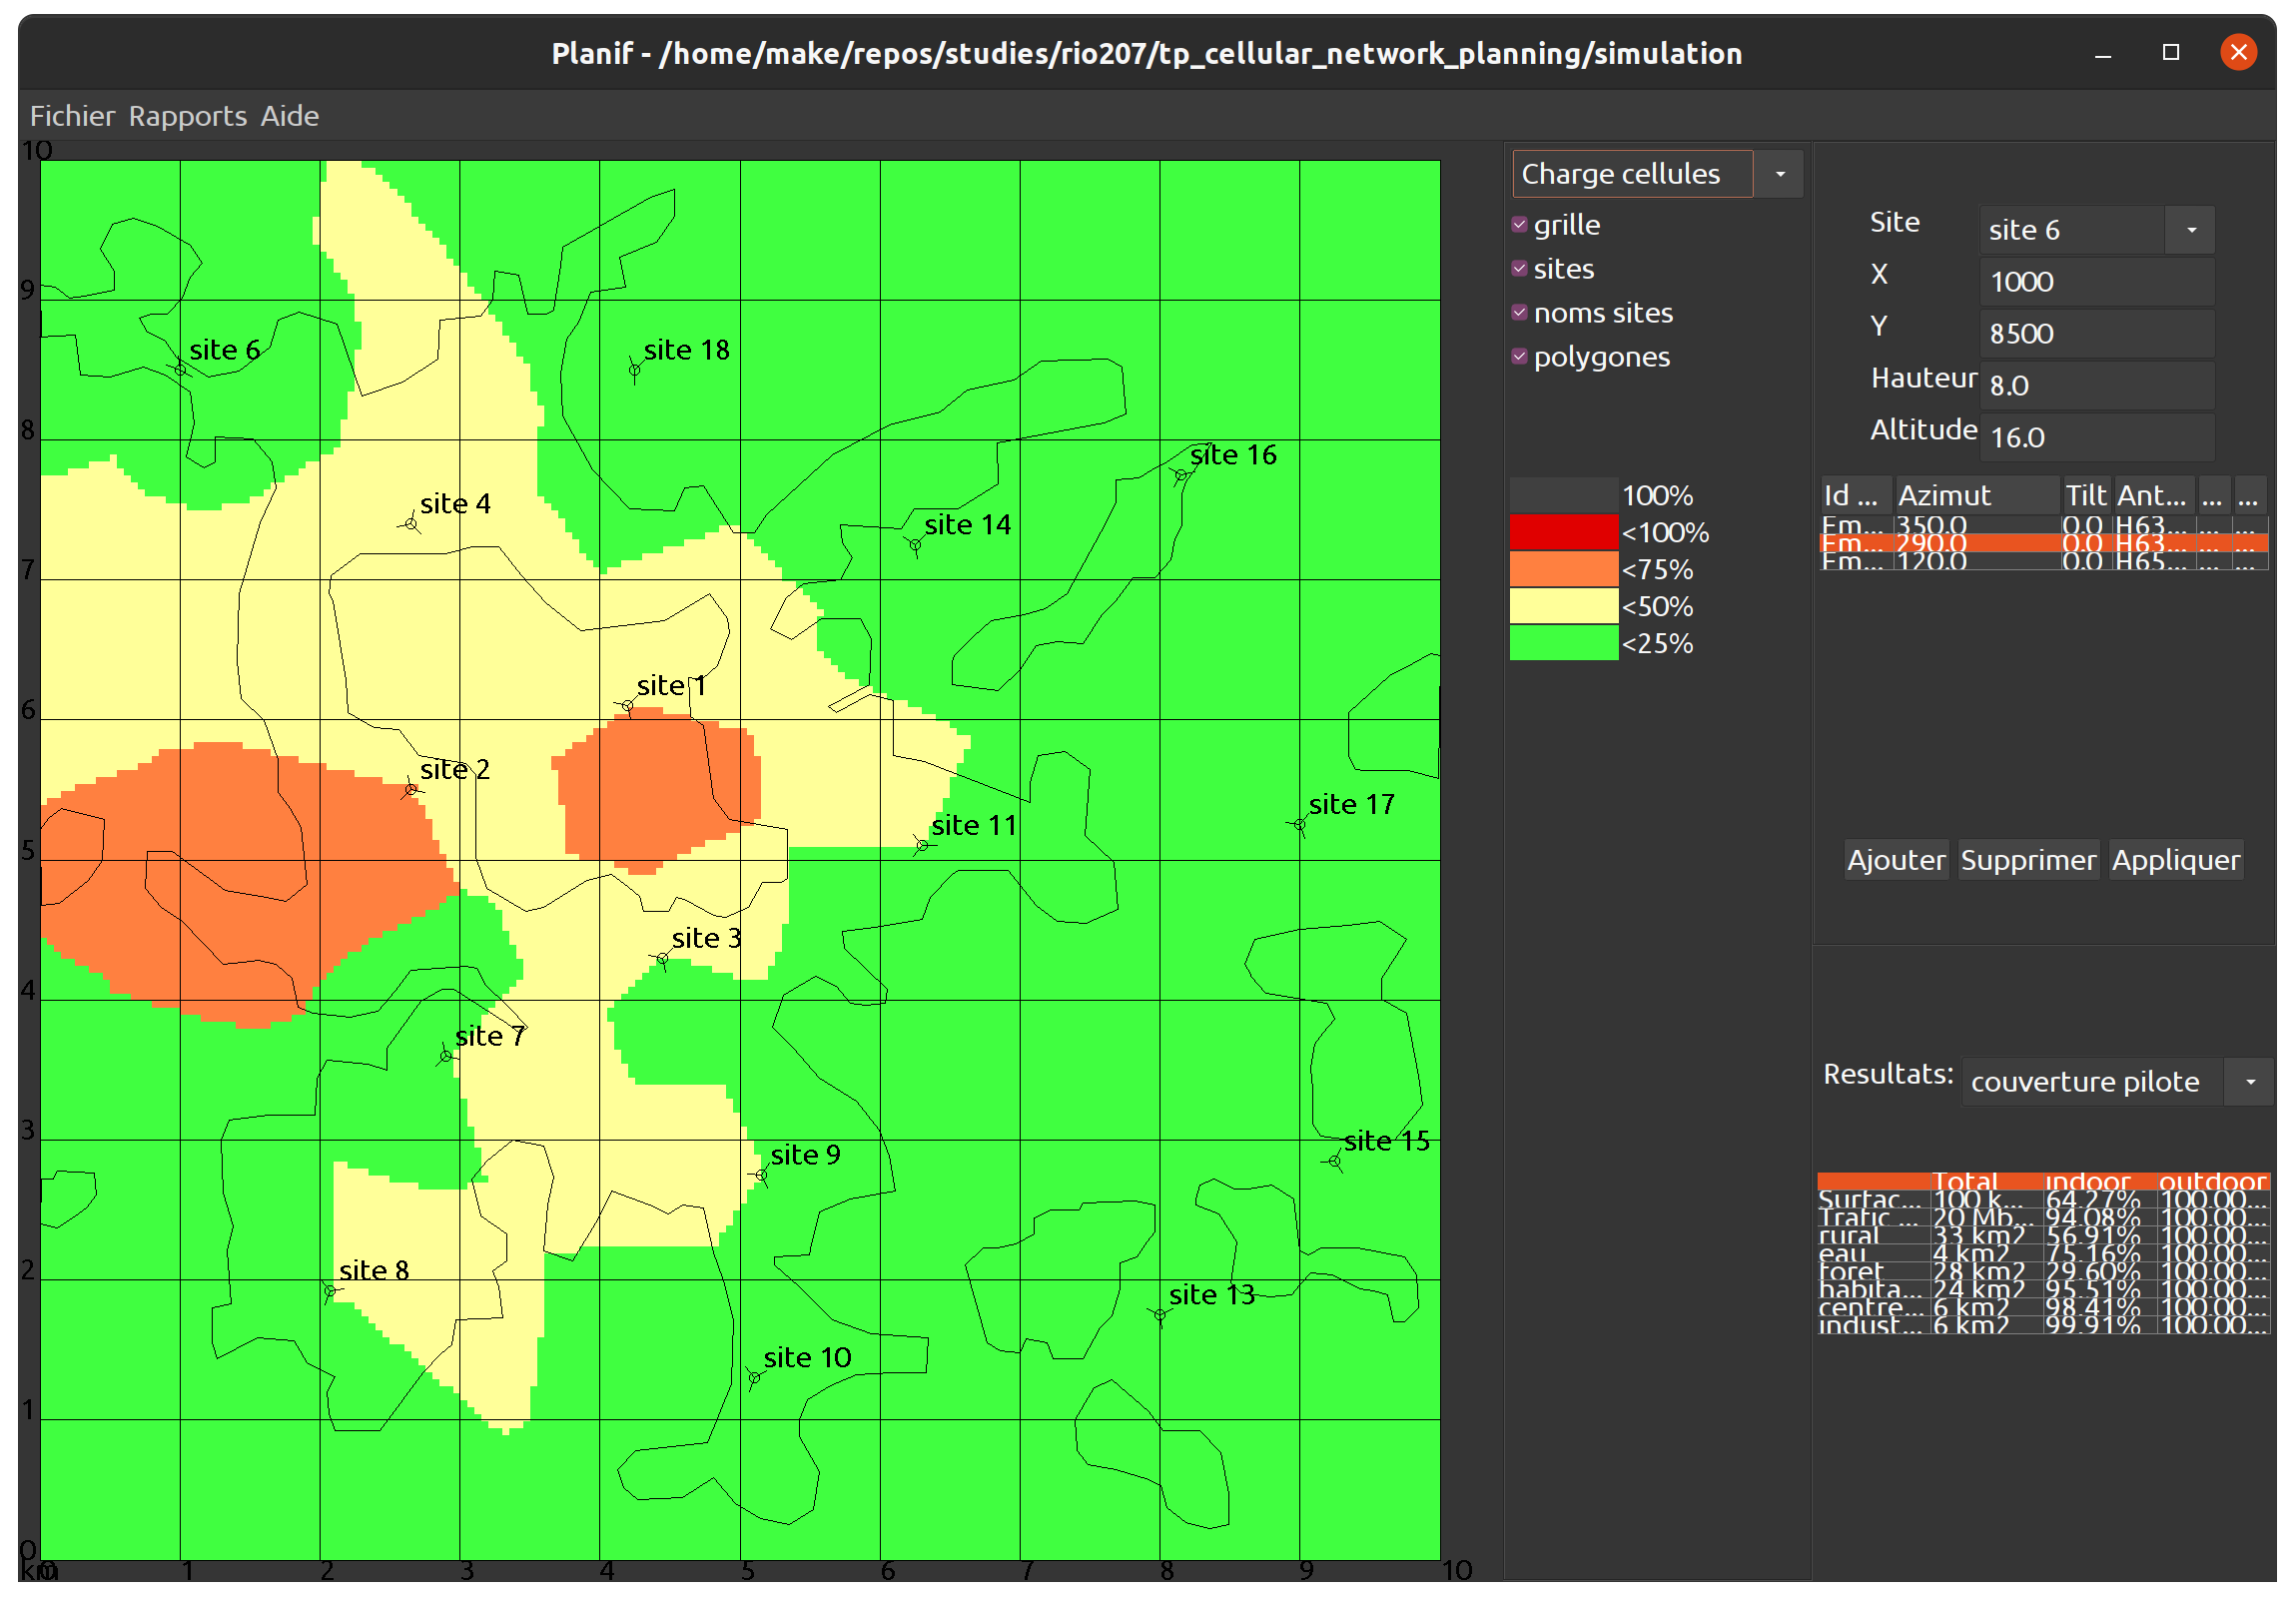
\includegraphics[width=12cm]{images/q8_cell_loading.png}
    \caption{Cell loading in the second deployment scenario.}
    \label{fig:q8_cell_loading}
\end{figure}


\end{document}

